\chapter{SYSTEM ANALYSIS AND DESIGN}

\section{System Analysis}
System analysis is a process of collecting and interpreting facts, identifying the problems, and decomposition of a system into its components.

\subsection{Requirement Analysis}
Requirement analysis focuses on the tasks that determine the needs or conditions to meet the new or altered product or project, taking account of the possibly conflicting requirements of the various stakeholders.

\subsubsection{Functional Requirements}
Functional requirements define the specific behavior or functions of the system.
\begin{enumerate}
    \item \textbf{Authentication:} Users must be able to register and login securely.
    \item \textbf{Expense Management:} Users can add, edit, and delete expenses using NLP text or manual forms.
    \item \textbf{Categorization:} The system automatically categorizes expenses using AI.
    \item \textbf{Visualization:} Users can view charts and graphs of their spending.
    \item \textbf{Group Expenses:} Users can create groups and split bills.
\end{enumerate}

\begin{figure}[H]
    \centering
    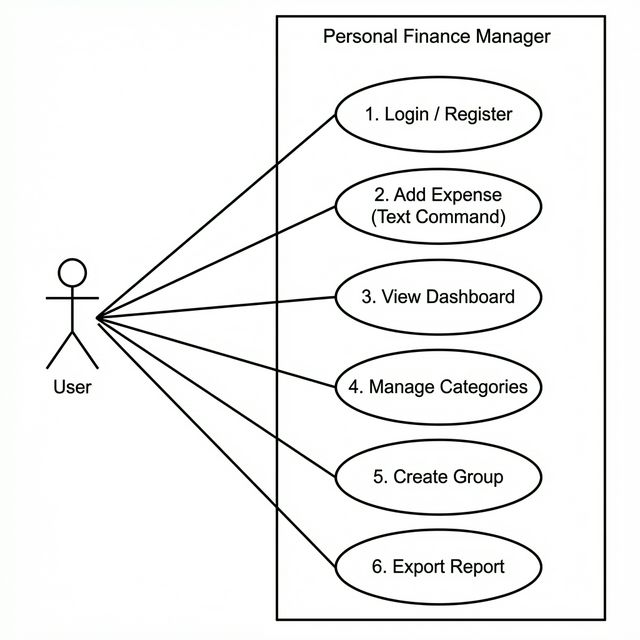
\includegraphics[width=0.8\textwidth]{images/use_case_diagram.png}
    \caption{Use Case Diagram}
    \label{fig:usecase}
\end{figure}

\subsubsection{Non-functional Requirements}
\begin{enumerate}
    \item \textbf{Performance:} Response time for NLP parsing should be under 2 seconds.
    \item \textbf{Reliability:} The system should be available 99.9\% of the time.
    \item \textbf{Security:} Passwords must be hashed; API communication must be over HTTPS.
    \item \textbf{Scalability:} System should handle concurrent users without degradation.
\end{enumerate}

\subsection{Feasibility Analysis}
\subsubsection{Technical Feasibility}
The project uses React (Frontend), Python FastAPI (Backend), and PostgreSQL (Database), which are mature technologies. The integration with Gemini API is supported by official libraries. Thus, the project is technically feasible.

\subsubsection{Operational Feasibility}
The interface is designed to be intuitive, resembling a chat application. No special training is required for users, making it operationally feasible.

\subsubsection{Economic Feasibility}
The project relies on open-source technologies and free-tier cloud services (Supabase, Vercel, Google AI Studio). The primary investment is development time, making it economically feasible.

\subsection{Data Modelling: ER Diagram}
Entity-Relationship (ER) diagram shows the relationships of entity sets stored in a database.

\begin{figure}[H]
    \centering
    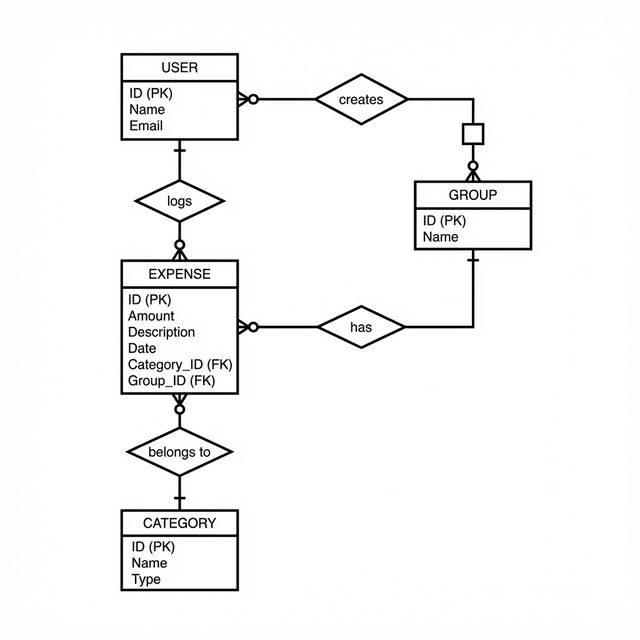
\includegraphics[width=0.9\textwidth]{images/er_diagram.png}
    \caption{Entity Relationship (ER) Diagram}
    \label{fig:er}
\end{figure}

\subsection{Process Modelling: DFD}
Data Flow Diagram (DFD) maps the flow of information for any process or system.

\begin{figure}[H]
    \centering
    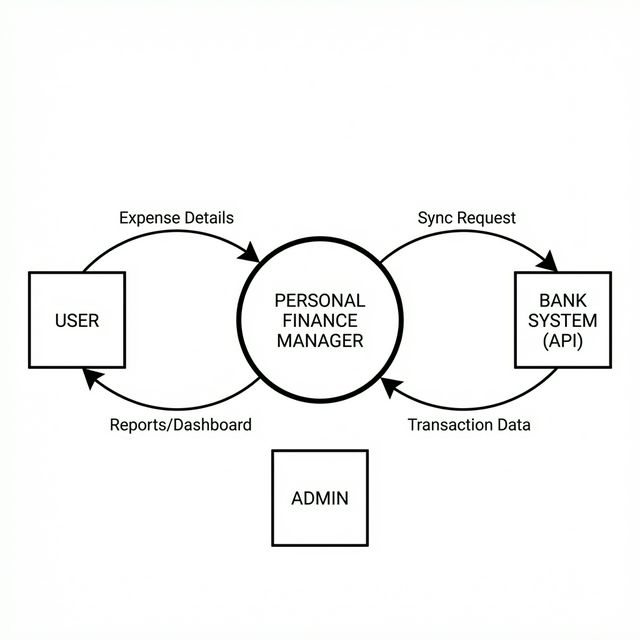
\includegraphics[width=0.9\textwidth]{images/dfd_diagram.png}
    \caption{Data Flow Diagram (Level 0)}
    \label{fig:dfd}
\end{figure}

\subsection{Object Modelling: Object \& Class Diagram}
Class diagram describes the structure of a system by showing the system's classes, their attributes, operations (or methods), and the relationships among objects.

\begin{figure}[H]
    \centering
    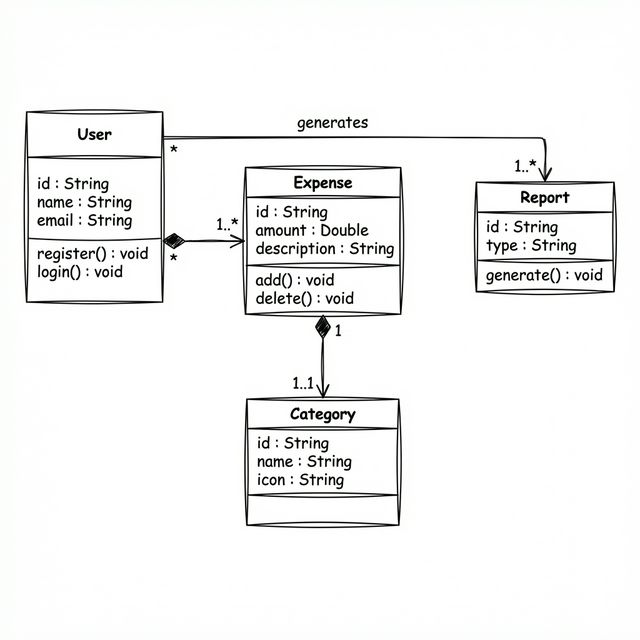
\includegraphics[width=0.9\textwidth]{images/class_diagram.png}
    \caption{Class Diagram}
    \label{fig:class}
\end{figure}

\subsection{Dynamic Modelling: State \& Sequence Diagram}
\subsubsection{State Diagram}
State diagram describes the behavior of a system.

\begin{figure}[H]
    \centering
    \includegraphics[width=0.6\textwidth]{images/state_diagram.png}
    \caption{State Diagram of Expense Processing}
    \label{fig:state}
\end{figure}

\subsubsection{Sequence Diagram}
Sequence diagram shows how objects operate with one another and in what order.

\begin{figure}[H]
    \centering
    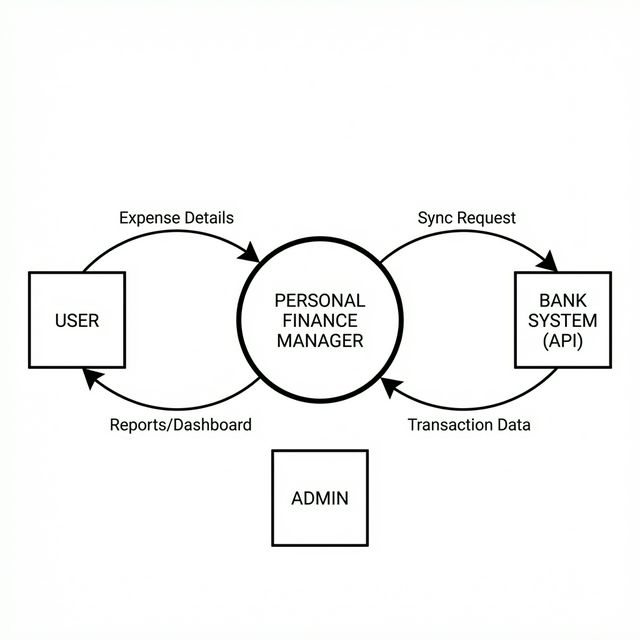
\includegraphics[width=0.9\textwidth]{images/sequence_diagram.png}
    \caption{Sequence Diagram for Adding Expense}
    \label{fig:sequence}
\end{figure}

\subsection{Process Modelling: Activity Diagram}
Activity diagram graphically represents workflows of stepwise activities and actions with support for choice, iteration, and concurrency.

\begin{figure}[H]
    \centering
    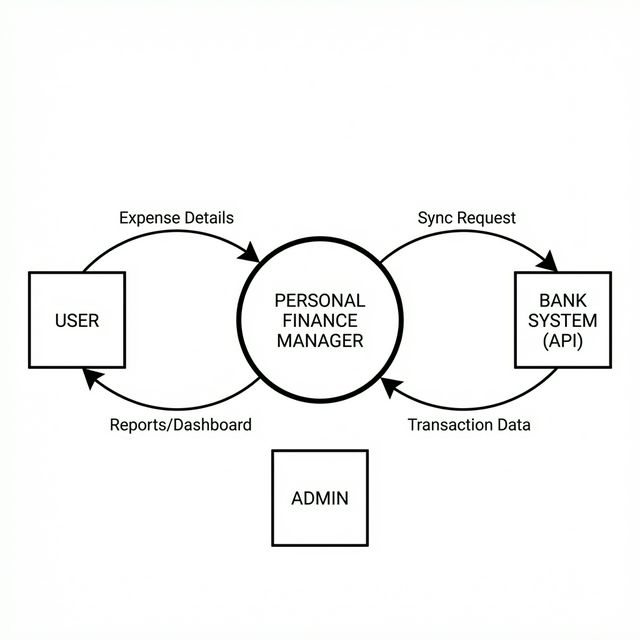
\includegraphics[width=0.6\textwidth]{images/activity_diagram.png}
    \caption{Activity Diagram}
    \label{fig:activity}
\end{figure}

\section{System Design}

\subsection{Architectural Design}
The system uses a \textbf{Client-Server Architecture}. The client is a React Single Page Application (SPA) wrapped in Capacitor for mobile. The server is a REST API built with FastAPI.

\subsection{Database Schema Design}
The database is normalized to 3NF.
\begin{itemize}
    \item \textbf{Users Table:} \texttt{id, restricted\_uid, email, full\_name, created\_at}
    \item \textbf{Categories Table:} \texttt{id, name, type, icon}
    \item \textbf{Expenses Table:} \texttt{id, amount, description, date, user\_id, category\_id, group\_id}
    \item \textbf{Groups Table:} \texttt{id, name, created\_by}
\end{itemize}

\subsection{Interface Design (UI/UX)}
The UI is designed for mobile-first usage. It features a bottom navigation bar, a central floating action button for adding expenses, and a card-based layout for listing transactions.

\subsection{Refinement of Classes and Object}
The initial class model was refined to include helper classes for API communication (\texttt{ApiService}) and state management (\texttt{ExpenseContext}).

\subsection{Component Diagram}
Component diagram depicts how components are wired together to form larger components or software systems.

\begin{figure}[H]
    \centering
    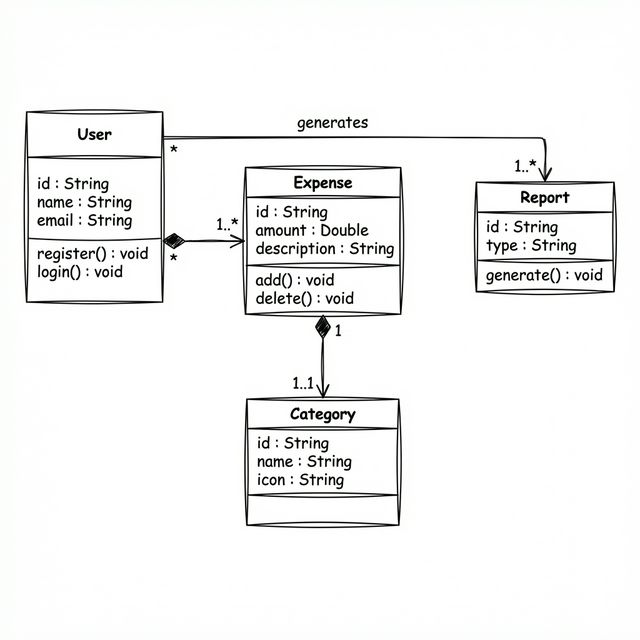
\includegraphics[width=0.7\textwidth]{images/component_diagram.png}
    \caption{Component Diagram}
    \label{fig:component}
\end{figure}

\subsection{Deployment Diagram}
Deployment diagram shows the physical hardware on which the software components run.

\begin{figure}[H]
    \centering
    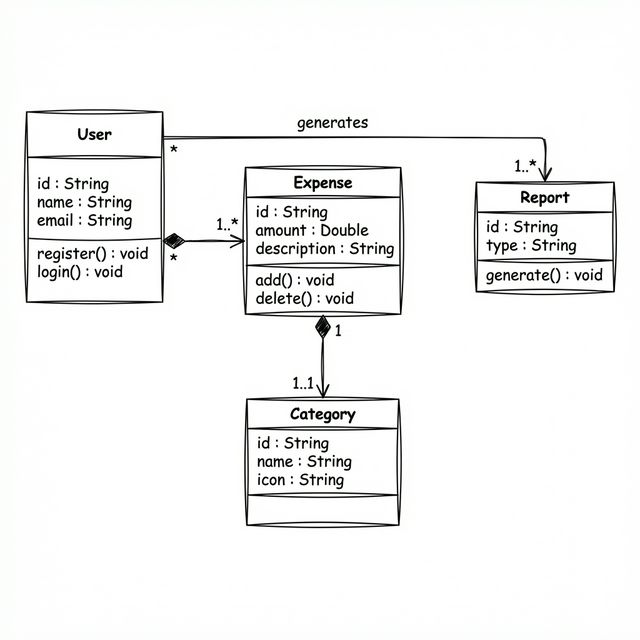
\includegraphics[width=0.7\textwidth]{images/deployment_diagram.png}
    \caption{Deployment Diagram}
    \label{fig:deployment}
\end{figure}

\section{Algorithm Details}
The NLP processing algorithm is central to the system:
\begin{enumerate}
    \item \textbf{Input:} Raw text string $S$ from user.
    \item \textbf{Tokenization:} Send $S$ to LLM with schema instruction.
    \item \textbf{Extraction:} LLM identifies entities: \textit{Amount}, \textit{Currency}, \textit{Category} (mapped to enum), \textit{Date} (relative to absolute).
    \item \textbf{Validation:} Backend defines Pydantic models to validate the JSON structure.
    \item \textbf{Output:} Structured `ExpenseCreate` object or Error.
\end{enumerate}
